


%%%%%%%%%%%%%%%%%%%%%%%%%%%%%%%%%%%%%%%%%%%
%%%%%%  STYLE 34
%%%%%%%%%%%%%%%%%%%%%%%%%%%%%%%%%%%%%%%%%%%

\cxset{
 name=CHAPTER,
 numbering=Roman,
 number font-size=\small,
 number font-family=\rmfamily,
 number font-weight=\normalfont,
 number before={},
 number position=rightname,
 chapter font-family=\sffamily,
 chapter font-weight=\normalfont,
 chapter font-size=\small,
 number after={},
 chapter before={},
 chapter after={\par},
 chapter color={black!90},
 number color=\color{black!90},
 title beforeskip={},
 title afterskip={\vspace{50pt}},
 title before=,
 title after={\par},
 title font-family=\normalfont,
 title font-color=\color{black!80},
 title font-weight=\normalfont,
 title font-size=\LARGE}

\section{Basic astronomical phenomena}

The interesting part of this style is that it uses roman numerals to display the counter that is in a different font than that used for the chapter name.
\medskip
\begin{figure}[ht]
\centering
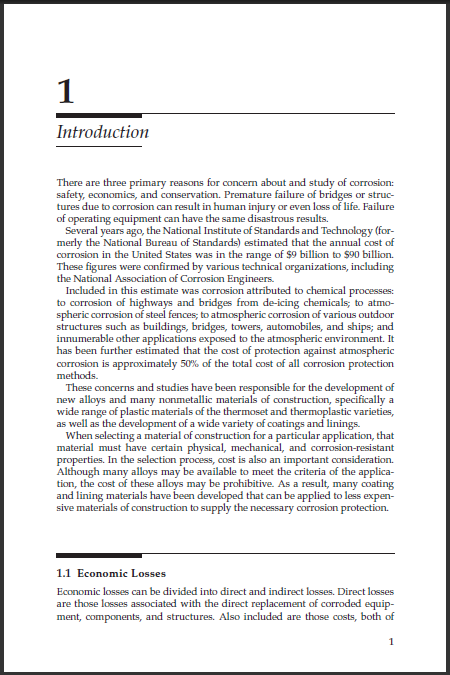
\includegraphics[width=0.6\textwidth]{./chapters/chapter34}
\end{figure}
